\documentclass[thesis.tex]{subfiles}
\begin{document}

\chapter{Prerequisites}\label{chap:preq}

\section{Earthquake Physics}\label{section:geophysikalische_grundlagen}
\subsection{The Earthquake Event}
An earthquake are caused by movements within the earth crust. These might result from earth plates moving under or against each other or artificial causes like mining works. After building up a lot of stress against friction, rock fractures along a fault line while the other tectonic layers can slip past each other. The fault line can even be visible on the surface. \\
The point where the fracturing starts is called hypocenter, while the epicenter is this point's projection onto the surface as seen in figure \ref{fig:hypocenter}. The breakage can extend to other points along the fault line as well as cause more ruptures.
\begin{figure*}[hb]
	\centering
	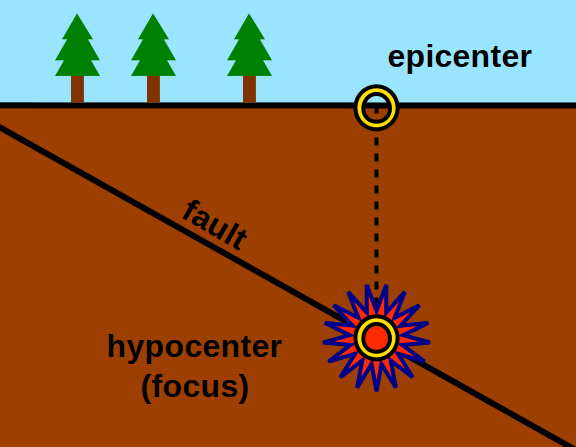
\includegraphics[width=0.6\linewidth]{../pictures/Prerequisites/Epicenter_Diagram.jpg}
	\caption{Hypocenter and Epicenter}
	\label{fig:hypocenter}
\end{figure*}
\subsection{Seismic Waves}
The energy, which is emitted as the fracturing occurs, travels through the earth crust as seismic waves. We denote different types of waves, which travel at different velocities. Soil and material type (air, liquid or solid) also affect wave arrival times. Waves also reflect on certain materials, creating many sub-types of waves to arrive.\\
The first wave to arrive at a site is the p-wave or primary/pressure wave. The propagating waves moves the material back and forth and is therefore also known as a compressional wave. \\
S-waves, second or shear waves move the material in a right angle to the movement direction. Contrary to p-waves, s-waves cannot move through liquid and are slightly slower than p-waves. Figure \ref{fig:speedwaves} shows this relationship.
\begin{figure*}[hb]
	\centering
	\includegraphics[width=0.6\linewidth]{../pictures/Prerequisites/Speeds_of_seismic_waves.PNG}
	\caption{Velocity of S and p Wave}
	\label{fig:speedwaves}
\end{figure*}
S-Wave and P-Waves are often denoted as body waves. Surface waves arrive even later and are the most damaging ones. Two important waves are Rayleigh and Love waves. Rayleigh waves cause the surface to "ripple", they move the ground up and down while Love waves cause horizontal shearing.
We can see all mentioned types of waves in figure \ref{fig:waves}.¸
\begin{figure*}[hb]
	\centering
	\includegraphics[width=0.6\linewidth]{../pictures/Prerequisites/waves.jpg}
	\caption{Overview of seismic waves}
	\label{fig:waves}
\end{figure*}
\section{Recording an Earthquake}
\subsection{Seismic Data}
The seismic waves which arrive on a site can be recorded by a seismometer, which is the instrument recording ground motion as displacement, velocity or acceleration. A seismograph is the system build around the seismometer. Seismograms show the measured motions as a 1D signal for the three motion orthogonal axes, namely north-south, east-west and ground-up. The recordings depend on the sensitivity of the sensors, but also on earthquake and location. For further reading see \cite{IntroEarthquakes}, page 398. An example for a recording of one axis at an earthquake arrival can be seen in figure \ref{fig:seismogram}. The change from noise to P-Wave to S-Wave arrival is clearly visible in the example. 
\subsection{Networks}
\subsection{Early Warning}
\begin{figure*}[hb]
	\centering
	\includegraphics[width=0.6\linewidth]{../pictures/Prerequisites/dia_seismogram.jpg}
	\caption{One axis recording of a seismograph}
	\label{fig:seismogram}
\end{figure*}
\section{Deep Learning foundations}
\subsection{Layers}
\subsection{Activation Functions}
\subsection{Improvement techniques}
\subsection{Regression and Classification tasks}
\section{Estimation Representation} 
 It is in important to keep in mind, that we do not take into account the uncertainty of our magnitude model and the representation of an earthquake with just ground motion sensors is itself a simplification.
\subsection{Types of uncertainty}
\subsection{Gaussian function}




\subfilebib % Makes bibliography available when compiling as subfile
\end{document}